% Template for SGN-3507 papers; to be used with:
%          spconf.sty   - ICASSP/ICIP LaTeX style file
%          IEEEtran.bst - IEEE bibliography style file

% Originally created for MCSP 20xx papers;
% Created:  Sep 2006 - Riku Uusikartano -- riku.uusikartano@tut.fi
% Modified: Sep 2007 - Riku Uusikartano -- riku.uusikartano@tut.fi
% Modified: Oct 2009 - Riku Uusikartano -- riku.uusikartano@tut.fi
% Modified: Oct 2010 - Jukka Suhonen -- jukka.suhonen@tut.fi
% Modified: Oct 2011 - Francescantonio Della Rosa -- francescantonio.dellarosa@tut.fi
% Modified: Nov 2011 - Jukka Suhonen -- juka.suhonen@tut.fi
% Modified for SGN-3507 March 2013 - Juha Pajula -- juha.pajula(a)tut.fi
% Modified for SGN-16006 Jan 2014 - Hanna Silen -- hanna.silen(a)tut.fi

% --------------------------------------------------------------------------
\documentclass{article}

% The amsmath and epsfig packages greatly simplify the process of adding
% equations and figures to the document, and thus their use is highly
% recommended.
% ------------
\usepackage{spconf,amsmath,epsfig}
\usepackage{subcaption}

% Title.
% ------
\title{Smile Recognition}

\name{Jesper Granat, Peter Todorov
%\thanks{Insert sponsor acknowledgments (where necessary) here.}
}
%
\address{jesper.granat@tuni.fi, peter.todorov@tuni.fi}

% Hyphenation (hyphenate all names and non-english words here).
% -------------------------------------------------------------
\hyphenation{Tam-pe-re micro-soft}

\begin{document}

\maketitle
\sloppy

% Abstract.
% ---------
\begin{abstract}
In this study, a convolutional neural network was trained to recognize
smile from an image. The training and deployment was done using the
Keras framework on top of the Tensorflow framework. The training data
was 4 000 images of smiling and non-smiling faces. The accuracy on
this dataset was 86,XXX \%.
\end{abstract}

% First section, often named as Introduction.
% -------------------------------------------
\section{Introduction}\label{sec:intro}
Since their introduction [REFERENCE], Convolutional Neural Networks
(CNNs) have been widely used in solving various image processing
problems, such as classification, object recognition and image
enhancement [REFERENCE]. In this study, a custom design CNN is trained
for real-time smile recognition. Real-time in this context refers to
inference speed where the network can be run on live video feed in
over 20 fps on a laptop with GPU\@.

\section{Background}\label{sec:background}
Convolutional Neural Networks (CNNs) have been shown to be essential in
modern computer vision applications, such as classification
[REFERENCE]. Classification in particular is rather difficult problem
due to its complexity. Here, the goal is to assign a label from a
predefined set of labels to an image. Difficulties in this task
include truncation of objects (object is partially not in the image),
occlusion of objects (some other object is blocking some parts of
the desired object), variations in color and lighting, and intra-class
variation. The complexity of classification can be intuitively
explained by considering a case where an image of a cat is desired to
be classified. The problem here is learning a representation of a cat,
as many cats can look different, an image of the same cat from
different angle and lighting yields in a completely different matrix
of pixel values in the image. [REFERENCE]

Traditional approaches to image classification have utilized
hand-crafted algorithms such Histogram of Oriented Gradients (HOG)
[REFERENCE]. In such algorithms, pixel color values and pixel
proximities are utilized to create a representation of the training
data. Since 2012 [REFERENCE], CNNs have been dominant in
classification. Particularly, deep CNNs from 2015 [REFERENCE] are
still dominant in classification. These can include hundreds or even
thousands of layers of convolutions. Typical CNNs for classification
include two types of layers: convolutional layers and pooling layers.
Pooling layers introduce non-linearity to the model to make is
feasible to include several layers of convolutions. Convolutional
layers, on the other hand, are responsible for creating the image
representation. The last layer(s) in CNNs are usually fully connected
layers. The output of the network are the probabilities of each class
being in the image.

CNNs for classification are trained with cross-entropy loss
[REFERENCE]. The idea of the loss is to punish weights that are
responsible for wrong classification, and reward weights that are
responsible for correct classification during training. Additionally,
batch normalization [REFERENCE] is used to generalaize the results.
Furthermore, classification with CNNs includes many more bells and
whistles that create the absolute best results.

\section{Solution}\label{sec:solution}
% 1. & 2.
The CNN model used in this study will be trained on GENKI-4K Face
dataset [REFERENCE]. In addition to the smile status, the training
data contains also the face orientation, but that will be ignored in
this study. It could be utilized to orient the faces upright as a
preprocessing step, but that is out of scope of this study. Therefore,
the problem to be solved in this study is formulated as a binary
classification problem. The data is split randomly into 80 \% training
data and 20 \% test data in a stratified manner. This means that both
splits contain equal proportions of positive and negative examples.

% 3.
The CNN archtecture used in this study is similar to the one proposed
in the laboratory instructions [REFERENCE], and it is implemented with
the Keras [REFERENCE] framework. In addition to the layers proposed by
the instructor, a batch normalization layer is added in front of every
convolutional layer. A $3 \times 3$ convolutional kernel is used in
every convolutional layer. Normally distributed glorot initializer
[REFERENCE] is used to initialize the kernel weights, and each layer
contains $L2$-regularization. The activation function for the fully
connected layer is Sigmoid activation [REFERENCE]. The model is
trained for 50 epochs using Adam [REFERENCE] optimizer and batch size
of 32. Otherwise the default Keras parameters are used.

% 4.
Finally, an additional sanity check and demonstrator is constructed by
reading a web camera feed in real time. Each frame is sent to the
model synchronously, and the output of the model is displayed in the
grafical user interface in a human-readable form. This functionality
is implemented with the OpenCV computer vision library [REFERENCE].

\section{Results}\label{sec:results}
The solution described in Section~\ref{sec:solution} was achieved
through iterative optimizion. First, the default parameters were used,
which gave a somewhat reasonable result. Batch normalization was then
added, because from our previous experience with neural networks we
knew it would help. It did improve the results a little bit. The
largest difference in this case, however, was achieved by carefully
selecting the loss function. Cross-entropy loss was noted to be the
superior loss for this case. Finally, when $L2$-regularization was
added, the model beat the desired accuracy.

\begin{table}[]
\centering
\caption{The confusion matrix for the optimized default architecture
  with batch normalization}\label{tab:default-confusion}
\begin{tabular}{lll}
\hline
                                 & Not smiling & Smiling \\ \hline
\multicolumn{1}{l|}{Not smiling} & 268         & 100     \\
\multicolumn{1}{l|}{Smiling}     & 65          & 367     \\ \hline
\end{tabular}
\end{table}

\begin{table}[]
\centering
\caption{The confusion matrix for the optimized 4 layer architecture
  with batch normalization and regularization (accuracy 0.86875 \%)}\label{tab:sixlayers}
\begin{tabular}{lll}
\hline
                                 & Not smiling & Smiling \\ \hline
\multicolumn{1}{l|}{Not smiling} & 309         & 59     \\
\multicolumn{1}{l|}{Smiling}     & 46          & 386     \\ \hline
\end{tabular}
\end{table}


\begin{figure}
  \centering
  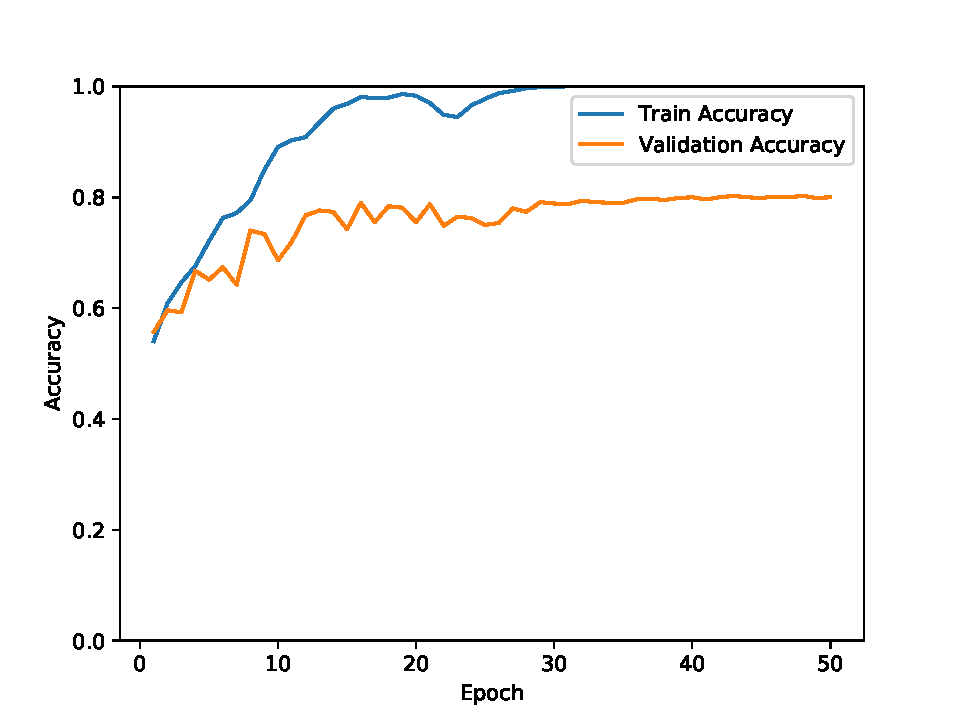
\includegraphics[width=\linewidth]{figures/default_bn.pdf}\label{fig:default}
  \caption{Learning curve with optimized hyperparameters and batch
    normalization with the default architecture}
\end{figure}


\section{Conclusion}\label{sec:conclusion}

\small

% IEEEtran is a LaTeX style file defining the reference formatting.
% -----------------------------------------------------------------
\bibliographystyle{IEEEtran}

% IEEEabrv is a LaTeX style file defining the abbreviations of different
% journals and conferences. mcsp_refs contains the actual reference data
% from which the references are selected into the paper using \cite{}.
% ----------------------------------------------------------------------

% Comment of following line if bibliography is not needed
%\bibliography{mcsp_refs}

% ---------------------------------------------------------------------------
\vfill\pagebreak

\end{document}

